 \documentclass[a4paper]{article}

\usepackage[a4paper]{geometry}
\usepackage{amssymb,amsmath}
\usepackage{amsthm}
\usepackage[utf8]{inputenc}
\usepackage{enumerate}
\usepackage{color}
\usepackage{graphicx}
\usepackage[estonian]{babel}
\usepackage[usenames,dvipsnames]{xcolor}
\usepackage{float}
\usepackage{cite}
\usepackage{etoolbox}
\usepackage{theoremref}
\usepackage[hidelinks]{hyperref}

\allowdisplaybreaks
\makeatletter
\patchcmd{\HyField@FlagsRadioButton}{\HyField@SetFlag{Ff}{Radio}}{}{}{}
\makeatother
\def\DefaultOptionsofRadio{print}



\definecolor{background_example}{HTML}{EDEDED}
%E0DCDE


\setlength\parindent{0pt}
\newenvironment{tightcenter}{%
  \setlength\topsep{0pt}
  \setlength\parskip{0pt}
  \begin{center}
}{%
  \end{center}
}

\author{Vootele Rõtov}
\title{Bakatöö}

\numberwithin{equation}{section}
\theoremstyle{definition}
\newtheorem{kumer_hulk}[equation]{Definitsioon}
\newtheorem{kumer_f}[equation]{Definitsioon}

\begin{document}

\maketitle

\pagebreak

\tableofcontents

\pagebreak

\section*{Spikker}

{\color{cyan} Helesinine- komentaarid}

{\color{blue} Tumesinine - asjad, mille õigsust peaks kontrollima}


{\color{cyan}\section*{Miks ma käesolevat asja teen?}

Panen kirja mõned põhjused, miks ma tegelen selle asjaga:
\begin{enumerate}[I]
\item Sellest on kellegile kasu - loodan realselt, et saan hakkama mingi toreda asjaga, millest keegi(näiteks Marguse psühholoogidest sõbrad) kasu saab.
\item Saab kätte selle paberi, mis teeb minust parema inimese. 
\item Midagi uut, olen juba päris pikalt tarkust ühes formaadis kuula õppejõudu, tööta läbi tema poolt valitud materjalid, esita see õppejõule, äkki selline formaat, kus tuleb ise otsida ja ise mõelda meeldib.
\item Väljakutse, kuigi viimaste aastatega on enesemotivatsioon kõvasti paranenud, ei ole see veel seal, kus ta olla võiks. Loodetavasti "treenin" seda aspekti.
\end{enumerate}}

\section{Töö \"ulesehitus}
Esiteks tutvustame lugejale vajalikku taustinfot, seejärel kirjeldame probleemip\"ustitust. Sellele järgneb töö eesmärgi matemaatiline p\"ustitus.

\section{Taustinfo}

\subsection{Likerti skaala
}
Käesolev uurimus tegeleb k\"usimustikega (\textit{Likert scale}), milles soovitakse hinnanguid teatud arvule väidetele (\textit{Likert item}) viie pallisel Likerti skaalal \cite{Edmondson}. Näiteks: \footnote{Näited terviklikest k\"usimustikest on lisades, \hyperref[likert1]{joonisel \ref*{likert1}} ja \hyperref[likert2]{ \ref*{likert2}}}

\vspace{10pt}

\begin{figure}[H]


\colorbox{background_example}{\parbox{\textwidth}{

\vspace{1mm}

Käesoleva bakalaureusetöö \"ulesehitus on loogiline.

\vspace{5pt}

\begin{Form}
\def\DefaultWidthofChoiceMenu{12pt}%



\ChoiceMenu[bordercolor = gray,disabled = true,name=optionE,radio,radiosymbol=\ding{108}]{\mbox{}}\null Ei nõustu 
\ChoiceMenu[bordercolor = gray,disabled = true,name=optionD,radio,radiosymbol=\ding{108}]{\mbox{}}\null Ei nõustu osaliselt
\ChoiceMenu[bordercolor = gray,disabled = true,name=optionC,radio,radiosymbol=\ding{108}]{\mbox{}}\null Nii ja naa
\ChoiceMenu[bordercolor = gray,disabled = true, name=optionB,radio,radiosymbol=\ding{108}]{\mbox{}}\null Nõustun osaliselt
\ChoiceMenu[bordercolor = gray,disabled = true,name=optionA,radio,radiosymbol=\ding{108}]{\mbox{}}\null Nõustun


\end{Form}}}
\caption{Näide väitest, millele palutakse hinnangut Likerti skaalal}
\label{likert_question}
\end{figure}

\paragraph{Likerti skaala -  järjestikskaala või intervallskaala?}\mbox{}\\*

Lugejal võib tekkida õigustatud k\"usimus, kuidas põhjendab autor Likerti skaala käsitlemist intervallskaalana, kui Likerti skaala oli algselt mõeldud järjestikskaalana ning  selle kasutamise osas intervallskaalana on autorid pigem skeptilised \cite{Jamieson2004}. Sellest hoolimata on intervallksaala tõlgendus praktikas piisavalt levinud, et selle valdkonna uurimine õigustatud oleks. Siinkohal vajab esile toomist, et kriitikute \"uks levinumaid argumente on see, et "`hea"'  ja "`väga hea"'  keskmine ei ole  loomulikul viisil tõlgendatav kui "`hea + pool"', millega autor ka nõustub ning loodab pakkuda sellele alternatiivset tõlgendust. 

\subsection{Valiidsus ja reliaablus}
Testi \textbf{valiidsus} on testi karakteristik, mis iseloomustab testi võimet mõõta seda, mida ta disainiti mõõtma. 
Testi \textbf{reliaablus} on testi omadust saada sama subjekti erinevatel mõõtmistel sama testiga sama tulemus. Järgnev joonis illustreerib reliaabluse ja valiidsuse mõisteid.

\begin{figure}[H]
\centering

\includegraphics[width=0.75\textwidth, height = 0.8\textwidth]{Reliability_and_validity.png}
\caption{Reliaabluse (\textit{reliability}) ja valiidsuse (\textit{validity}) omavahelist suhestumine.  \cite{Dilmen2008}}
\label{reliability_and_validity}
\end{figure}

On selge, et testi kõrge valiidsus on vajalik tingimus selleks, et test oleks kasutatav h\"upoteesi kontrolliks või mingite järelduste tegemiseks. Teoreetiliselt on võimalik ps\"uhhomeetriline test, mille valiidsus on suur ja reliaablus väike, kui eeldada et mõõtmisviga on sõltumatu juhuslik suurus, eeldus mida ka tavaliselt tehakse. Intuitiivselt on selge, et selline test ei praktikas kasutatav, kuna me ei oska väheste mõõtmiste raames hinnata mõõtmisvigade suurust ning piisavalt suure arvu mõõtmiste teostamine ei ole reaalselt võimalik, seega on praktikas testi kõrge reliaablus vajalik tingimus testi kõrgeks valiidsuseks.    

\subsection{Reliaabluse formaalne definitsioon}
Definitsioon andmisel võtame aluseks Melvin Novicki klassikalisest testiteooria \cite{Novick1966}\cite{Lord1968} tõlgendusest \cite[109]{Sijtsma2009}. 

Olgu meil mingi kogum $I$ testile vastajaid ning mingisugune test, milles on $k$ k\"usimust ning olgu $X_{i}^{j}$ juhuslik suurus, mille jaotusfunktsioon sõltub vastajast, mille võimalike väärtusi vaatleme kui k\"usimuse $j$ vastuse arvulist tõlgendust mingi vastaja $i$ jaotusele vastavalt. Defineerime vastaja $i$ testi tulemuse $X_{+i}$ kui 

\begin{equation*}
X_{+i} = \sum \limits_{j=1}^k X_{i}^{j} \text{.}
\end{equation*}


Kuna juhusliku suuruste summa on samuti juhuslik suurus {\color{cyan} Okey lugeda juhuslik suurus selliseks mõisteks, mida ei ole vaja defineerida?} siis on $X_{+j}$ juhuslik suurus, mille jaotusfunktsioon on vastajast sõltuv.
Analoogiliselt võime vaadelda ka testi tulemusi \"ule kõigi vastajate - sellisel juhul olgu $X^{j}$ juhuslik suurus mida iseloomustav jaotusfunktsioon kirjeldab kuidas vastajate populatsioon vastab k\"usimusele $j$  ning testi tulemus $X$ on defineeritav kui

\begin{equation*}
X = \sum \limits_{j=1}^k X^{j} \text{.}
\end{equation*}

Defineerime k\"usimuse tegeliku tulemuse vastaja $i$ jaoks kui testi tulemuse keskväärtuse {\color{cyan} Vajalik def ? } ehk

\begin{equation*}
t_i = \epsilon  \left[ X_{+i} \right] \text{.}\footnote{Tähistame keskväärtuse tähega $\epsilon$ kuna tavapärane tähistus $E$ leiab antud käsitluses teistsuguse rolli.}
\end{equation*}

Paneme tähele, et vaadeldes tegeliku tulemust \"ule kõigi vastajate võime rääkide tegelikust tulemusest kui juhuslikust suurusest, mida tähistame $T$ ja mille võimalike väärtuste hulk on $\left\lbrace t_i ~ | ~ i \in I \right\rbrace$.

Tõlgendame vastaja $i$ testi tulemuse ja tegeliku tulemuse vahet mõõtmisveana, tähistame seda $E_i$. Seega $X_{+i} = t_i + E_i$. Analoogiliselt saame tõlgendada viga \"ule kõigi vastajate kui juhusliku suurust $E$, kusjuures $X = T + E$.

Paneme tähele, et eelneva põhjal on vastaja $i$ mõõtmisvea keskväärtus $0$. Tõepoolest, kuna tegeliku tulemuse definitsiooni põhjal $\epsilon \left[ X_{+i} \right] = t_i$, siis saame mõõtmisvea definitsiooni arvesse võttes 
\begin{equation*}
 t_i = \epsilon \left[ X_{+i} \right] = \epsilon \left[ t_i + E_i \right] = \epsilon \left[ t_i \right] + \epsilon \left[ E_i \right] = t_i + \epsilon \left[ E_i \right] \implies \epsilon \left[ E_i \right] = 0 \text{.}
\end{equation*}

Lisaks on lihtne märgata, et  $D \left[ X_i \right] = D \left[ E_i \right]$, sest 
\begin{equation*}
D \left[ X_i \right] = D \left[ E_i + t_i \right] = D \left[ E_i \right] \text{.}
\end{equation*}  

Eelnevates definitsioonides keskendusime testi tulemuste mõtestamisele fikseeritud vastaja korral, tuues paralleelselt sisse analoogilised mõisted \"ule mingi vastajate kogumi. Kuna reeglina mõtestatakse teste praktikas mingi vastajate kogumi raames, siis keskendume ka meie edaspidi sellele.

Niisiis, olgu meil meli mingi vastajate kogum $I$ ja eespool kirjeldatud juhuslikud suurused $X,T,E$, kusjuures $X = T + E$.


Järgevalt esitame neli keskset klassikalise testi teooria eeldust \cite[10]{DeGruijter2005}:
\begin{enumerate}[I]
\item mõõtmisvea keskväärtus \"ule vastajate populatsiooni on 0 ehk 
\begin{equation*}
\epsilon \left[ E \right] = 0 \text{,}
\end{equation*}
\item korrelatsioon {\color{cyan} Def vajalik?} mõõtmisvea ja tegeliku tulemuse vahel \"ule vastajate kogumi on $0$ ehk
\begin{equation*}
corr \left( T, E \right) = 0 \text{.}
\end{equation*} 
\item Olgu meil sama testi kaks erinevat mõõtmist \"ule vastajate kogumi $I$, mille tulemused on $X$ ja $X`$, kusjuures $X = T + E$ ja $X` = T` + E`$. Siis \"uhe mõõtmise tegelik tulemus ei korreleeru teise mõõtmisveaga ehk
\begin{equation*}
corr \left( T, E' \right) = 0 \text{,}
\end{equation*}   
\item lisaks sellele ei korreleeru ka erinevate mõõtmiste mõõtmisvead ehk
\begin{equation*}
corr \left( E, E' \right) = 0 \text{.}
\end{equation*}
\end{enumerate}

Järgnevalt toome sisse paralleelse testi mõiste. Kaks testi, mille tulemused \"ule kõigi vastajate kogumi $I$ on $X$ ja $X'$ on paralleelsed parajasti siis, kui kehtivad järgmised väited :
\begin{enumerate}
\item $t_i = t_i' ~ \forall i \in I$
\item $D \left[ X \right] = D \left[ X' \right]$ {\color{cyan} Dispersiooni definitsioon vajalik ? }
\end{enumerate}



Paralleelse testi abil saame klassikalise testiteooria raames defineerida reliaabluse. Olgu meil kaks paralleelselt testi, mille tulemused \"ule vastajate kogumi $I$ on vastavalt $X$,$X'$ kus kumbgi ei ole konstante juhuslik suurus. Testi, mille tulemus on $X$,  reliaablus \"ule vastajate kogumi $I$ on võrdne $X$ ja $X'$ korrelatsiooniga (Pearsoni mõttes), mida tähistame $\rho_{XX'}$, formaalselt

{\color{cyan}korrelatsiooni (ja kovariatsiooni definistioonid vajalikud?}
\begin{equation*}
\rho_{XX'} = corr \left( X,X' \right) \text{.}
\end{equation*} 

Paralleelse testi definitsiooni ja klassikalise testiteooria eelduste põhjal kehtib \begin{gather*}
\rho_{XX'} = \frac{cov(XX')}{\sqrt{D \left[ X \right] D \left[ X' \right]}} =   
\frac{\epsilon \left[XX' \right] - \epsilon \left[X \right] \epsilon \left[ X' \right]}{D \left[ X \right]} = \\ 
= \frac{\epsilon \left[\left(T + E \right) \left( T' + E ' \right) \right] - \epsilon \left[T + E \right] \epsilon \left[ T'+E' \right]}{D \left[ X \right]} = \\
= \frac{\epsilon \left[\left(T + E \right) \left( T + E ' \right) \right] - \left( \epsilon \left[T \right] - \epsilon \left[ E \right] \right) \left( \epsilon \left[ T \right] - \epsilon \left[ E' \right] \right)}{D \left[ X \right]} = \\
= \frac{\epsilon \left[T^2 + TE + TE' + EE'  \right] -  \epsilon \left[T \right]  \epsilon \left[ T \right]}{D \left[ X \right]} = \\
= \frac{\epsilon \left[T^2 \right]  + \epsilon \left[ TE \right] + \epsilon \left[ TE' \right] + \epsilon \left[ EE'  \right] -  \epsilon \left[T \right]^2}{D \left[ X \right]} 
= \frac{\epsilon \left[T^2 \right] - \epsilon \left[ T \right]^2}{D \left [ X \right] } = \\ 
= \frac{cov(T,T)}{D \left[ X \right]} = \frac{D \left[T \right]}{D \left[ X \right]} \text{.}
\end{gather*}

Paneme tähele, et eelneva põhjal $\rho_{XX'} \in \left[0,1 \right]$. Samuti märgime, et kuna $T = X - E$, siis kehtib
\begin{equation*}
\rho_{XX'} = \frac{D \left[ T \right]}{D \left[ X \right] } = \frac{D \left[ X - E \right]}{D \left[ X \right] } = \frac{D \left[X \right] - D \left[ E \right]}{D \left[ X \right]} = 1 - \frac{D \left[ E \right]}{D \left[ X \right]} \text{.}
\end{equation*}

Eelneva põhjal on selge, et väide  "testi reliaablus on suurem" on samaväärne järgmise kolme väitega\cite[110]{Sijtsma2009}:
\begin{enumerate}
\item testi korrellatsioon paralleelse testiga on suurem,
\item testi tegeliku tulemuse dispersioon on suurem võrreldes testi tulemuse dispersiooniga,
\item testi mõõtmisvea dispersioon on väiksem võrreldes testi tulemuse dispersiooniga.
\end{enumerate}

Märgime, et klassikalise testiteooria raames defineeritud reliaablus sobib kokku paragraafi alguses antud mitteformaalse definitsiooniga, kuna paralleelseks testiks võib lugeda ka sama testi uuesti läbiviimise sama vastajate kogumi peal, kusjuures klassikalise testiteooia eeldused ei ole väga kitsendavad, kui suudame tagada selle, et testis ei esine s\"usteematilisi mõõtmisvigu. 

Kuna testi tegelik tulemus on suurus, mida me prakikas ei tea ning ka paralleelsete testide läbiviimine ei ole tihti võimalik on kasutusele võetud mitmeid praktikas kasututavaid hinnanguid, mis on reliaabluse alumisteks tõketeks. Järgnevalt vaatleme mõningaid neist.
 
Reliaabluse mõõtmise viisidest on osutunud popularseimaks sisemise reliaabluse leidmine, näiteks kolm neljandikku Ameerika \"Uhendriikide teadusajakirjas "`\textit{Directory of Unpublished Experimental Mental Measures}"' ilmunud uurimustest kasutas testi reliaabluse hindamiseks justnimelt sisemist reliaablust \cite[177] {Henson2001}. Järgnevalt vaatleme  seda reliaabluse mõõtmise viisi lähemalt. 


\subsection{Sisemine reliaablus}

K\"usimustiku sisemine reliaablus (\textit{internal consistency}) hindab testi erinevate k\"usimuste vastuste järjepidevust ehk seda, kui hästi on kooskõlas \"uhist  konstruktsiooni hindavad k\"usimused\cite[177] {Henson2001}. Piltlikult väljendudes, olgu meil järgnev k\"usimustik: 

\begin{figure}[H]

\colorbox{background_example}
	{\parbox
		{\textwidth}
			{
			\setlength{\unitlength}{1mm}
			\begin{picture}(148,55)
				\put(0,52){Käesolevat bakalaureusetööd on lihte lugeda.}
				\put(0,47){\line(1,0){14}}
				\put(8,41){Ei nõustu}
				\put(16,47){\circle{4}}
				\put(16,47){\circle*{2}}
				\put(18,47){\line(1,0){25}}
				\put(32,41){Ei nõustu osaliselt}
				\put(45,47){\circle{4}}
				\put(45,47){\circle*{2}}
				\put(47,47){\line(1,0){25}}
				\put(67,41){Nii ja Naa}
				\put(74,47){\circle{4}}
				\put(74,47){\circle*{2}}
				\put(76,47){\line(1,0){25}}
				\put(92,41){Nõustun osaliselt}
				\put(103,47){\circle{4}}
				\put(103,47){\circle*{2}}
				\put(105,47){\line(1,0){25}}
				\put(126,41){Nõustun}
				\put(132,47){\circle{4}}
				\put(132,47){\circle*{2}}
				\put(134,47){\vector(1,0){14}}
				\put(0,32){Mulle meeldib käesoleva bakalaureusetöö \"ulesehitus.}
				\put(0,27){\line(1,0){14}}
				\put(8,21){Ei nõustu}
				\put(16,27){\circle{4}}
				\put(16,27){\circle*{2}}
				\put(18,27){\line(1,0){25}}
				\put(32,21){Ei nõustu osaliselt}
				\put(45,27){\circle{4}}
				\put(45,27){\circle*{2}}
				\put(47,27){\line(1,0){25}}
				\put(67,21){Nii ja Naa}
				\put(74,27){\circle{4}}
				\put(74,27){\circle*{2}}
				\put(76,27){\line(1,0){25}}
				\put(92,21){Nõustun osaliselt}
				\put(103,27){\circle{4}}
				\put(103,27){\circle*{2}}
				\put(105,27){\line(1,0){25}}
				\put(126,21){Nõustun}
				\put(132,27){\circle{4}}
				\put(132,27){\circle*{2}}
				\put(134,27){\vector(1,0){14}}
				\put(0,12){Käesoleva bakalaureusetöö \"ulesehitus on loogiline.}
				\put(0,7){\line(1,0){14}}
				\put(8,1){Ei nõustu}
				\put(16,7){\circle{4}}
				\put(16,7){\circle*{2}}
				\put(18,7){\line(1,0){25}}
				\put(32,1){Ei nõustu osaliselt}
				\put(45,7){\circle{4}}
				\put(45,7){\circle*{2}}
				\put(47,7){\line(1,0){25}}
				\put(67,1){Nii ja Naa}
				\put(74,7){\circle{4}}
				\put(74,7){\circle*{2}}
				\put(76,7){\line(1,0){25}}
				\put(92,1){Nõustun osaliselt}
				\put(103,7){\circle{4}}
				\put(103,7){\circle*{2}}
				\put(105,7){\line(1,0){25}}
				\put(126,1){Nõustun}
				\put(132,7){\circle{4}}
				\put(132,7){\circle*{2}}
				\put(134,7){\vector(1,0){14}}
			\end{picture}
		}
		
	}
\caption{K\"usimustik bakalaureusetöö \"ulesehituse kohta }
\label{quiz_consistency}
\end{figure}

Siin on mõõdetavaks konstruktsiooniks käesoleva bakalaureusetöö \"ulesehitus ning sisemiseks reliaabluseks on vajalik kolmele näites toodud k\"usimusele antud vastuste kooskõla.



\subsection{Cronbachi alfa}

Cronbachi alfa on levinud sisemist reliaablust iseloomustav näitaja, mis on defineeritud järgnevalt:

\begin{equation}
(\frac{k}{k-1})( 1 - \frac{\sum \sigma_i^2}{\sigma_t^2})
\end{equation}

kus $k$ tähistab k\"usimuste arvu, $\sigma_i$ on standardviga \"uhe k\"usimuse piires ja $\sigma_t$ on standardviga \"ule testi kogutulemuste.\cite[396]{Cronbach2004}

{\color{cyan} Siia selgitav näidis tabel/joonis vajalik?}


\paragraph{Miks ma taandan selles töös sisemise järjekindluse mõõtmise Cronbachi alfale?}\mbox{}\\*

Kuna Cronbach'i alfal on mitmeid puuduseid, millest mõningad on toodud ära David Streineri artiklis \cite[101-102]{Streiner2010}, ning isegi mõõdiku autor Lee Cronbach soovitab oma 1951. aastal välja töötatud mõõdiku asemel kasutatada alternatiivseid mõõdikuid \cite{Cronbach2004}, on oluline vastata alapealkirjas p\"ustitatud k\"usimusele. Kaks peamist põhjust on järgnevad:
\begin{enumerate}[I]
\item Cronbachi alfa on hetkel kõige kasutatavam mõõdik sisemise reliaabluse mõõtmiseks ps\"uhho-meetriliste testide juures. Seetõttu on väljapakutud meetod testide tulemuste anal\"u\"usijatele tuttav ning seega loodetavasti lihtsamini kasutatav.
\item Cronbachi alfa leidmine on arvutuslikult k\"ullaltki lihtne. Kuna käesoleva töö peamine eesmärk on selgitada, kas väljapakutud lähenemine on mõistlik, siis ei ole parematest mõõdikutest potentsiaalselt saadav kasu piisavalt suur, et tasa teha \"ulesande lahendamise raskemaks muutumist. Juhul, kui töö tulemus on aga positiivne,  tuleks uurida ka teiste mõõdikute võimalikku kasutamist.

\end{enumerate}

\paragraph{Milliseid piiranguid seab Cronbachi alfa kasutamine?}\mbox{}\\*

Tooksin esile kaks tähtsamat piirangut:
\begin{enumerate}[I]
\item Uuritavate k\"usimustike puhul peaks sama konstruktsiooniga tegelema võimalikult palju k\"usimusi, vältima peaks k\"usimustikke, kus \"uhe konstruktsiooni kohta on alla kolme k\"usimuse.
\item K\"usimustikud ei tohi olla liiga pikad, Cronbachi alfa peegeldab lisaks sisemisele järjekindlusele ka k\"usimustiku pikkust. \cite[101]{Streiner2010} Liiga pika k\"usimustiku puhul on oht, et pikkusest saab domineerv osa Cronbachi alfast.
\end{enumerate}

\label{sec:Cronbach}









\section{\"Ulesande p\"ustitus}

Selle töö raames loodame välja pakkuda viisi, kuidas paigutada intervallskaalal erinevaid vastuseid Likerti skaalalt. Eesmärk on leida parem paigutus kui vaikimisi meetod, kus eeldatakse, et erinevate hinnagute vahekaugused on samad. Vaatleme kahte näidet:


\begin{figure}[H]


\colorbox{background_example}
	{\parbox
		{\textwidth}
			{
			\setlength{\unitlength}{1mm}
			\begin{picture}(148,15)
				\put(0,12){Käesoleva bakalaureusetöö \"ulesehitus on loogiline.}
				\put(0,7){\line(1,0){14}}
				\put(8,1){Ei nõustu}
				\put(16,7){\circle{4}}
				\put(16,7){\circle*{2}}
				\put(18,7){\line(1,0){25}}
				\put(32,1){Ei nõustu osaliselt}
				\put(45,7){\circle{4}}
				\put(45,7){\circle*{2}}
				\put(47,7){\line(1,0){25}}
				\put(67,1){Nii ja Naa}
				\put(74,7){\circle{4}}
				\put(74,7){\circle*{2}}
				\put(76,7){\line(1,0){25}}
				\put(92,1){Nõustun osaliselt}
				\put(103,7){\circle{4}}
				\put(103,7){\circle*{2}}
				\put(105,7){\line(1,0){25}}
				\put(126,1){Nõustun}
				\put(132,7){\circle{4}}
				\put(132,7){\circle*{2}}
				\put(134,7){\vector(1,0){14}}
			\end{picture}
		}
		
	}
\caption{Näide, kuidas hinnangud skaalal hetkel vaikimisi meetodit kasutades paigutuvad}
\label{quiz}
\end{figure}

\begin{figure}[H]


	\colorbox{background_example}
	{\parbox
		{\textwidth}
			{
			\setlength{\unitlength}{1mm}
			\begin{picture}(148,15)
				\put(0,12){Käesoleva bakalaureusetöö \"ulesehitus on loogiline.}
				\put(0,7){\line(1,0){8}}
				\put(2,1){Ei nõustu}
				\put(10,7){\circle{4}}
				\put(10,7){\circle*{2}}
				\put(12,7){\line(1,0){18}}
				\put(19,1){Ei nõustu osaliselt}
				\put(32,7){\circle{4}}
				\put(32,7){\circle*{2}}
				\put(34,7){\line(1,0){20}}
				\put(49,1){Nii ja Naa}
				\put(56,7){\circle{4}}
				\put(56,7){\circle*{2}}
				\put(58,7){\line(1,0){33}}
				\put(82,1){Nõustun osaliselt}
				\put(93,7){\circle{4}}
				\put(93,7){\circle*{2}}
				\put(95,7){\line(1,0){30}}
				\put(121,1){Nõustun}
				\put(127,7){\circle{4}}
				\put(127,7){\circle*{2}}
				\put(129,7){\vector(1,0){19}}
			\end{picture}
		}
	}

\caption{Näide hinnangute alternatiivsest paiknemisest skaalal}
\label{quiz1}

\end{figure}

Kui me tahame välja pakkuda alternatiive vaikimisi hinnangule, peab meil olema põhjendus, miks välja pakutud lahendus kirjeldab reaalsust täpsemalt. Pakume välja järgmise lahenduse: 
\"uritame leida hinnangute paiknemist skaalal nii, et k\"usitluse sisemine reliaablus oleks võimalikult suur. Piirame ennast sellega, et  hinnangute esialgne järjestus ei tohi muutuda. Sisemise järjekindluse maksimeerimise taandame antud töö käigus Cronbachi alfa maksimeerimisele.\footnote{Põhjendus, miks selline taandamine on tehtud, on ära toodud peat\"ukis \hyperref[sec:Cronbach]{\ref*{sec:Cronbach}}.} 
 

\section*{Altervatiivid}

{\color{cyan} Ilmselt siit edasi ei lähe, lendab praeguses lahenduses välja (kui just mingi vahva idee peale ei tule). Võib-olla pakkuda siin välja alternatiive Cronbach'i alfa abil sobivate vahekauguste leidmisele) }
\begin{enumerate}
\item Kõige triviaalsem viis: kujutame kõikide k\"usimuste vastused hulgale $\left\lbrace 1,2,3,4,5 \right\rbrace$ , leiame mudeli, mille võime kirjeldada valitud k\"usimust on suurim. Tegemist on ilmselt vaikimisi variandiga ehk loodud mudelit peab võrdlema 
\item Selle asemel, et kujutada hulgale $\left\lbrace 1,2,3,4,5 \right\rbrace$, leiame sobivad vasted nii, et mudeli kirjeldav jõud oleks suurim. Sellise lähenemise oht seisneb selles, et meie mudel kirjeldab väga hästi olemasolevat valimit, kuid ei \"utle suurt midagi \"uldkogumi kohta. {\color{blue} Huvitav oleks, kas lihsalt nii midagi teha ei annaks ? Overfittimise vastu saaks, aga vaja oleks valimit, mis oleks piisavalt suur, et seda kaheks jagada(midagi, mille pealt mudelit ehitada ja midagi, mille pealt seda validifitseerida}. 
\item {\color{blue} Midagi veel? Peab uurima.}
\end{enumerate}

\section{\"Ulesande matemaatiline p\"ustitus}

Olgu meil k\"usimustik $n$-väitega, kus iga näite kohta palutakse hinnangut 5-palli Likerti skaalal. Hinnanguid võime vaadelda kui juhuslikke suurusi $K_1,K_2,...,K_n, K_iw$ mille muutumispiirkonnaks on hulk $\{1,2,3,4,5\}$. Toome sisse ka tähistused $p_{i \alpha}, i \in \{1,2,...,n\}, \alpha \in \{1,2,3,4,5\}$, kus $p_{i \alpha}$ tähistab olemasolevate andmete põhjal antud hinnangut tõenäosusele, et k\"usimusele $K_i$ anti hinnang $\alpha$. 

Tuletame meelde Cronbachi alfa definitsiooni:


\begin{equation*}
(\frac{k}{k-1})( 1 - \frac{\sum \sigma_i^2}{\sigma_t^2})
\end{equation*}

Paneme tähele, et toodud eelduste põhjal avalduks vaadeldava k\"usimustiku korral alfa järgnevalt:

 
\begin{equation*}
(\frac{k}{k-1})( 1 - \frac{\sum \sigma_i^2}{\sigma_t^2}) = \frac{n}{n-1}\left(1 - \frac
{\sum \limits_{i=0}^n D(K_i)}{D(\sum \limits_{i=0}^n K_i)}\right)
\end{equation*}

Võttes arvesse, et $D(\sum \limits_{i=0}^n K_i) = \sum \limits_{i=0}^n \sum \limits_{j=0}^n COV(K_i,K_j)$ saame eelneva kirjutada järgnevalt:

\begin{equation*}
(\frac{k}{k-1})( 1 - \frac{\sum \sigma_i^2}{\sigma_t^2}) = \frac{n}{n-1}\left(1 - \frac
{\sum \limits_{i=0}^n D(K_i)}{\sum \limits_{i=0}^n \sum \limits_{j=0}^n COV(K_i,K_j)}\right)
\end{equation*}
Vastavalt \"ulesande p\"ustituses toodud ideele soovime leida sellise viisi hinnangute tõlgendamiseks, et Cronbachi alfa oleks maksimaalne. Kujutame juhuslikud suurused $K_1,K_2,...,K_n$ juhuslikeks suurusteks $L_1, L_2,L_2,...,L_n$, kusjuures juhusliku suuruse $L_i$ määramispiirkond \"uhtib suuruse $K_i$ määramispiirkonnaga ning $L_i$ saab väärtusi hulgast $\Lambda_i = \{\lambda_{1i},\lambda_{2i},\lambda_{3i},\lambda_{4i},\lambda_{5i}\} ~ i \in {1,2,...n}$. Lisaks kehtigu järgnevad kitsendused: 


\begin{equation*}
\lambda_{i1} < \lambda_{i2}  < \lambda_{i3} < \lambda_{i4} < \lambda_{i5}
\end{equation*}

{\color{cyan} Siin peavad ikka ranged võrratused olema ,(0,0,0,0,1) ei kõlba.}

\begin{equation*}
K_i = 1 \implies L_i = \lambda_{i1}, K_i = 2 \implies L_i = \lambda_{i2},\cdots, K_i = 5 \implies L_i =\lambda_{i5}
\end{equation*}

Paneme tähele, et Cronbachi alfa arvutamine, seega ka maksimeerimine, on endiselt keeruline. Siinkohal märgime, et hinnangute tõlgenduste juures ei huvita meid mitte absoluutne, vaid suhteline paigutus. Niisiis võime juhuslikke suurusi piirata järgnevate kitsendustega:


\begin{equation}
E(L_i) = p_{i1}*\lambda_{i1}+p_{i2}*\lambda_{i2}+p_{i3}*\lambda_{i3}+
p_{i4}*\lambda_{i4}+p_{i5}*\lambda_{i5}=0
\end{equation}

\begin{equation}
D(L_i) = 
p_{i1}*(\lambda_{i1})^2+ p_{i2}*(\lambda_{i2})^2 + p_{i3}*(\lambda_{i3})^2 + p_{i4}*(\lambda_{i4})^2 + p_{i5}*(\lambda_{i5})^2 = 1 
\end{equation}


Paneme tähele, et sellisel skaalal olevaid k\"usimusi sisaldava testi Cronbachi alfa esitub lihtsamal kujul:

\begin{equation}
\alpha = \frac{n}{n-1}\left(1 - \frac
{n}{\sum \limits_{i=0}^n \sum \limits_{j=0}^n COV(L_i,L_j)}\right)
\end{equation}

Siit näeme, et sellisel juhul taandub Cronbachi alfa maksimeerimine avaldise $\sum \limits_{i=0}^n \sum \limits_{j=0}^n COV(L_i,L_j)$ maksimeerimisele. {\color{cyan} Järgev on täiesti trivaalne mapping Y = (X+1)*2 +1 vms. Põhjus miks ta siia sisse tõin oli soov rõhutada absoluutse skaala ebaolulisust. Võib välja jääda.}Kuna uuritavaid teste vaadeldakse tavaliselt 5-palli skaalal, siis pärast sobivate kordajate leidmist võime teha veel \"uhe teisenduse, mis viib vahemikkust $(-1,1)$ vahemikku $(0,5)$, säilitades hinnangute (mida oleme tähistanud $\lambda$-dega) omavaheliste kauguste suhte. {\color{cyan} normeerime } 

Kogu eelnevalt tehtud illustreerib järgmine joonis, kus autor on p\"u\"udnud selgitada \"uhe juhusliku suuruse määramispiirkonna muutuse läbi eelnevalt kirjeldatud protsesside. 

\begin{figure}[H]

\colorbox{background_example}
	{\parbox
		{\textwidth}
			{
			\setlength{\unitlength}{1mm}
			\begin{picture}(148,55)
				\put(0,52){Käesoleva bakalaureusetöö \"ulesehitus on loogiline.}
				\put(0,47){\line(1,0){14}}
				\put(15,41){1}
				\put(16,47){\circle{4}}
				{\color{violet}\put(16,47){\circle*{2}}}
				\put(18,47){\line(1,0){25}}
				\put(44,41){2}
				\put(45,47){\circle{4}}
				{\color{blue}\put(45,47){\circle*{2}}}
				\put(47,47){\line(1,0){25}}
				\put(73,41){3}
				\put(74,47){\circle{4}}
				{\color{green}\put(74,47){\circle*{2}}}
				\put(76,47){\line(1,0){25}}
				\put(102,41){4}
				\put(103,47){\circle{4}}
				{\color{yellow}\put(103,47){\circle*{2}}}
				\put(105,47){\line(1,0){25}}
				\put(131,41){5}
				\put(132,47){\circle{4}}
				{\color{red}\put(132,47){\circle*{2}}}
				\put(134,47){\vector(1,0){14}}
				
				
				
				\put(74,39){\vector(0,-1){9}}
				
				
				\put(21,27){\line(1,0){11}}
				\put(23,21){-1}
				
				\put(34,27){\circle{4}}
				{\color{violet}\put(34,27){\circle*{2}}}
				\put(31,21){-0.8}				
				
				\put(36,27){\line(1,0){31}}
				
				\put(69,27){\circle{4}}
				{\color{blue}\put(69,27){\circle*{2}}}
				\put(66,21){-0.1}	
				
				\put(71,27){\line(1,0){6}}
				
				\put(73,21){0}
				
				\put(79,27){\circle{4}}
				{\color{green}\put(79,27){\circle*{2}}}
				\put(77,21){0.1}	
				
				\put(81,27){\line(1,0){6}}
				
				\put(89,27){\circle{4}}
				{\color{yellow}\put(89,27){\circle*{2}}}
				\put(87,21){0.3}	
				
				\put(91,27){\line(1,0){6}}
				
				
				\put(99,27){\circle{4}}
				{\color{red}\put(99,27){\circle*{2}}}
				\put(97,21){0.5}	
				
				\put(101,27){\vector(1,0){24}}
				
				\put(123,21){1}
				
				
				\put(74,19){\vector(0,-1){9}}
				
				
				\put(0,7){\line(1,0){25.6}}
				\put(15,1){1}
				
				
				\put(27.6,7){\circle{4}}
				{\color{violet}\put(27.6,7){\circle*{2}}}
				\put(29.6,7){\line(1,0){36.5}}
				
				\put(44,1){2}
				
				\put(68.1,7){\circle{4}}
				{\color{blue}\put(68.1,7){\circle*{2}}}
				
				\put(70.1,7){\line(1,0){7.7}}
				
				\put(73,1){3}
				
				\put(79.8,7){\circle{4}}
				{\color{green}\put(79.8,7){\circle*{2}}}
				
				\put(81.8,7){\line(1,0){7.6}}
				\put(102,1){4}
				
				
				\put(91.4,7){\circle{4}}
				{\color{yellow}\put(91.4,7){\circle*{2}}}
				
				\put(93.4,7){\line(1,0){7.6}}
				\put(131,1){5}
				
				\put(103,7){\circle{4}}
				{\color{red}\put(103,7){\circle*{2}}}
				\put(105,7){\vector(1,0){43}}
				
				
				
			\end{picture}
		}
		
	}
\caption{Illustratsioon sellest, kuidas suhestub hulk $ran(K_i)$ hulka $ran(L_i)$ ning see omakorda hulka, mis tekib peale teisendust hulgast $ran(L_i)$ 5-palli skaalale, säilitades hinnagute vahelised kaugused  }
\label{projection}
\end{figure}


Olgu meil tõenäosuste maatriks $P$:
\begin{tightcenter}
\begin{equation*}
P =
\begin{pmatrix}
p_{(11)(11)}&p_{(11)(12)}&p_{(11)(13)}&p_{(11)(14)}&p_{(11)(15)}&p_{(11)(21)}&\cdots&p_{(11)(n5)} \\
p_{(12)(11)}&p_{(12)(12)}&p_{(12)(13)}&p_{(12)(14)}&p_{(12)(15)}&p_{(12)(21)}&\cdots&p_{(12)(n5)} \\
\vdots&\vdots&\vdots&\vdots&\vdots&\vdots&\ddots&\vdots \\
p_{(n5)(11)}&p_{(n5)(12)}&p_{(n5)(13)}&p_{(n5)(14)}&p_{(n5)(15)}&p_{(n5)(21)}&\cdots&p_{(n5)(n5)} \\
\end{pmatrix} 
\end{equation*}
\end{tightcenter}

kus  $p_{(i \alpha) (j \beta)}, i,j \in \{1,2,...,n\}, \alpha , \beta \in \{1,2,3,4,5\}$ tähistab tõenäosust, et k\"usimusele $K_i$ anti vastus $\alpha$ ja k\"usimusele $K_j$ anti vastus $\beta$. 

Paneme tähele, et kuna $p_{(i \alpha)( i \alpha)} = p_{i \alpha}$, siis avaldub eelnev maatriks ka järgnevalt:

\begin{tightcenter}
\begin{equation*}
P =
\begin{pmatrix}
p_{i \alpha}&p_{(11)(12)}&p_{(11)(13)}&p_{(11)(14)}&p_{(11)(15)}&p_{(11)(21)}&\cdots&p_{(11)(n5)} \\
p_{(12)(11)}&p_{i \alpha}&p_{(12)(13)}&p_{(12)(14)}&p_{(12)(15)}&p_{(12)(21)}&\cdots&p_{(12)(n5)} \\
\vdots&\vdots&\vdots&\vdots&\vdots&\vdots&\ddots&\vdots \\
p_{(n5)(11)}&p_{(n5)(12)}&p_{(n5)(13)}&p_{(n5)(14)}&p_{(n5)(15)}&p_{(n5)(21)}&\cdots&p_{i \alpha}\\
\end{pmatrix} 
\end{equation*}
\end{tightcenter}


Defineerime  vektori $x$:

\begin{tightcenter}
\begin{equation*}
x = (\lambda_{11},\lambda_{12},\lambda_{13} ,\lambda_{14},\lambda_{15},\lambda_{21},\lambda_{22},\lambda_{23},\lambda_{24},\lambda_{25}, \cdots ,\lambda_{n1},\lambda_{n2},\lambda_{n3},\lambda_{n4},\lambda_{n5})
\end{equation*}
\end{tightcenter}


Siis $xPx^T = \sum \limits_{i=1}^n \sum \limits_{j=1}^n COV(L_i,L_j)$. Veendume selles:
\begin{tightcenter}
\begin{equation*}
\begin{gathered}
xPx^T =
\begin{pmatrix}
\lambda_{11} & \lambda_{12} & \cdots & \lambda_{n5} 
\end{pmatrix}
\begin{pmatrix}
p_{(11)(11)}&p_{(11)(12)}&\cdots&p_{(11)(n5)} \\
p_{(12)(11)}&p_{(12)(12)}&\cdots&p_{(12)(n5)} \\
\vdots&\vdots&\ddots&\vdots \\
p_{(n5)(11)}&p_{(n5)(12)}&\cdots&p_{(n5)(n5)} \\
\end{pmatrix} 
\begin{pmatrix}
\lambda_{11} \\
\lambda_{12} \\
\vdots \\
\lambda_{n5}
\end{pmatrix}
= \\
= 
\begin{pmatrix}
\sum \limits_{j=1}^n \sum \limits_{l=1}^5 \lambda_{jl}p_{(jl)(11)}& \sum \limits_{j=1}^n \sum \limits_{l=1}^5 \lambda_{jl}p_{(jl)(12)} & \cdots &  \sum \limits_{j=1}^n \sum \limits_{l=1}^5 \lambda_{jl}p_{(jl)(n5)} \\
\end{pmatrix}
\begin{pmatrix}
\lambda_{11} \\
\lambda_{12} \\
\vdots \\
\lambda_{n5}
\end{pmatrix}
=\\
=
\sum \limits_{j=1}^n \sum \limits_{l=1}^5 \lambda_{jl}p_{(jl)(11)} + \sum \limits_{j=1}^n \sum \limits_{l=1}^5 \lambda_{jl}p_{(jl)(12)} + \cdots +  \sum \limits_{j=1}^n \sum \limits_{l=1}^5 \lambda_{jl}p_{(jl)(n5)}=\\
= \sum \limits_{i=1}^{n} \sum \limits_{k=1}^{5} \sum \limits_{j=1}^n \sum \limits_{l=1}^5 \lambda_{jl}p_{(jl)(ik)} \lambda_{ik} 
= \sum \limits_{i=1}^{n}  \sum \limits_{j=1}^n \sum \limits_{k=1}^{5} \sum \limits_{l=1}^5 \lambda_{jl}p_{(jl)(ik)} \lambda_{ik} =
\sum \limits_{i=1}^{n} \sum \limits_{j=1}^n E(L_iL_j) = \\
\underset{(1)}{=} \sum \limits_{i=1}^{n} \sum \limits_{j=1}^n E(L_iL_j) - E(L_i)E(L_j) = \sum \limits_{i=1}^{n} \sum \limits_{j=1}^n COV(L_i,L_j)
\end{gathered}
\end{equation*}
\end{tightcenter}


Eelneva põhjal piisab meile Cronbachi alfa leidmiseks ruutvõrrandi $xPx^T$ maksimeerimisest, arvestades eelnevalt äratoodud piiranguid $L_i$ keskväärtusele ja dispersioonile..
Selle põhjal saame p\"ustitada  \textit{Quadratically constrained quadratic programm(QCQP)}'i {\color{cyan}Mingi pädev eestikeelne termin selle kohta ?} t\"u\"upi optimeerimisprobleemi, mille lahendus annab meile otsitavad tõlgendused. Teeme seda:  



\begin{gather}
min ~ x^T(-P)x  \notag \\
R_i^Tx = 0,  i \in {1,2,...,n} \notag \\
 R_i = (\underbrace{0,0,...0,0}_{(i-1)*5}p_ia,p_ib,p_ic,p_id,p_ie, \underbrace{0,0,...,0,0}_{(n-i)*5})  \displaybreak[1] \\
x^TP_ix = 1, i \in \{1,2,...,n\}, ~
P_i =
\begin{pmatrix}
p_{ja}&0&\cdots &0 \\
0&p_{jb}&\cdots &0 \\
\vdots & \vdots & \ddots & \vdots \\
0&0&\cdots & p_{je} \\
\end{pmatrix} \notag \\
p_j\alpha = 
\begin{cases} 
0 &  j \neq i  \\ 
p_i\alpha & i = j 
\end{cases}
, \alpha \in \{a,b,c,d,e\} \notag
\end{gather}

\section{Ülesande t\"u\"ubi keerekuse anal\"u\"us}
Järgnevas anal\"u\"usime ruutkitsendustega ruuplaneerimis\"ulesannete keerukust \"uldisemalt. Kõigepealt defineerime \"uldkuju, selleks on,
\begin{equation}
\begin{gathered}
\label{QCQP}
min~ \frac{1}{2}x^T P_0 x + q_0^Tx  \\
\frac{1}{2}x^T P_i x + q_i^Tx + r_i \leq 0 , i \in \left\lbrace 1,...,m \right\rbrace, \\
Ax = b, P_0,P_i \in R^{n \times n}, x,q_0,q_i \in R^{n}, \text{kus x on optimeeritav muutuja.} 
\end{gathered}
\end{equation}
Paneme tähele, et kitsendused $x_i(x_i-1) \leq 0 $, $x_i(1-x_i) \leq 0 $ rahuldavad probleemi  \eqref{QCQP} kitsendustele pandud tingimusi. Tõepoolest, toodud kitsendused saab viia kujule
\begin{equation*}
\begin{gathered}
x^TP_i x + (-q_i^T) x \leq 0, \\
x^T(-P_i)x + q_i^Tx \leq 0, P_i =
\begin{cases}
p_ii = 1 \\ 
p_jk = 0, j,k \neq i
\end{cases}, 
q_i = \begin{cases}
q_i = 1 \\
q_j = 0, j \neq i
\end{cases}.
\end{gathered}
\end{equation*}
Eelnevad kitsendused on samaväärsed kitsendusega $x_i(x_i-1) = 0$, mis on samaväärne kitsendusega $x_i \in \left\lbrace 0,1 \right\rbrace$. Niisiis saab kahendtäisarv-programmi (binary integer program, 0-1 integer program) esitada eelnevalt kirjeldatud kujul.

\subsection{Kahendtäisarv programm}
 Kahendtäisarv-programm on optimeerimisprobleem, kus kõik muutujad peavad saama väärtusi hulgast $\left\lbrace 0,1 \right\rbrace$. Kahendtäisarv-programmi kanooniline kuju on 
\begin{equation}
\begin{gathered}
\label{binary}
max~ c^T x \\
Ax \leq b, \\
x_i \in  \left\lbrace 0,1 \right\rbrace, \\
a \in A, b_0 \in  b, c_0 \in c \implies a,b_0,c_0 \in \mathbb{Z} 
\end{gathered}
\end{equation}

\subsection{NP-Hard probleemid}

\section{\"Ulesande anal\"u\"usiks vajalik taust}
\subsection{Kumerus}
\begin{kumer_f}
Olgu 
\end{kumer_f}

\section{Lahenduse idee}
{\color{cyan} Kas probleem on SDP t\"u\"upi või SDP? Miidlale kirjutan vast nendes k\"usimustes. Mingi sissejuhatav jutt QCQP ja SDP kohta, kas algusessse taust peat\"ukki või pigem teksti sisse ?}
P\"ustitatud optimeerimis probleemi lahendamiseks teisendame probleemi \textit{semidefinite programming(SDP)} t\"u\"upi optimeerimis\"ulesandeks ning seejärel lahendame saadud \"ulesande.

\section{Teisendus \textit{QCQP} t\"u\"upi \"ulesandelt \textit{SDP} t\"u\"upi \"ulesandele}

Esiteks teisendame saadud \textit{QCQP} standartkujule. {\color{cyan} Siia vaja selgitusi, mis ja kuidas}

\begin{gather}
min ~ -\theta  \notag \\
x^T P x -\theta \leq 0 \notag \\
R_i^Tx \leq 0,  i \in {1,2,...,n} \notag \\
-R_i^Tx \leq 0,  i \in {1,2,...,n} \notag \\
 R_i = (\underbrace{0,0,...0,0}_{(i-1)*5}p_ia,p_ib,p_ic,p_id,p_ie, \underbrace{0,0,...,0,0}_{(n-i)*5})  \displaybreak[1] \\
x^T P_i x - 1 \leq 0, i \in \{1,2,...,n\} \notag \\
-(x^T P_i x - 1) \leq 0, i \in \{1,2,...,n\} \notag \\
P_i =
\begin{pmatrix}
p_{ja}&0&\cdots &0 \\
0&p_{jb}&\cdots &0 \\
\vdots & \vdots & \ddots & \vdots \\
0&0&\cdots & p_{je} \\
\end{pmatrix} \notag \\
p_j\alpha = 
\begin{cases} 
0 &  j \neq i  \\ 
p_i\alpha & i = j 
\end{cases}
, \alpha \in \{a,b,c,d,e\} \notag
\end{gather}\cite[116]{Epelman2007}
 
Paneme tähele, et kuna maatriksid $P,R_i,P_i$ on s\"ummeetrilised ja mittenegatiivselt määratud, siis  leiduvad maatrikisd $Q,S_i,Q_i$ nii, et $P = QQ^T, R_i= S_i S_i^T, P_i = Q_i Q_i^T$. Nende maatriksite leidmiseks saab kasutada Cholesky lahutust.   \cite[151]{Tammeraid1999} {\color{cyan}raamatus juhj positiivselt määratud maatriksi korral, mittenegatiivselt määratud maatriksi korral sellied maatriksid leiduvad, kuid ei ole alati \"uheselt määratud.}

Olgu A mittenegatiivselt määratud maatriks, olgu $A = LL^{T}$.Märkame,  et kehtib järgnev:

\begin{equation}
\label{quadric_to_semidef}
x^T A x \leq b^T x + c \iff \begin{pmatrix}
I_k & L^T x \\
x^T L & b^Tx+c \\
\end{pmatrix} \succeq 0
\end{equation}\cite[31]{Laurent2012}

Seega saame anda oma optimeerimisprobleemile järgneva kuju:

\begin{gather}
min ~ -\theta  \notag \\
\begin{pmatrix}
I_k & Q^Tx \\
x^T Q & \theta \\
\end{pmatrix} 
\succeq 0 \notag \\
R_i^Tx \leq 0,  i \in {1,2,...,n} \notag \\
-R_i^Tx \leq 0,  i \in {1,2,...,n} \notag \\
 R_i = (\underbrace{0,0,...0,0}_{(i-1)*5}p_ia,p_ib,p_ic,p_id,p_ie, \underbrace{0,0,...,0,0}_{(n-i)*5})  \displaybreak[1] \\
\begin{pmatrix}
I_k & Q_i^Tx \\
t^T & 1 \\
\end{pmatrix} \succeq 0 \notag \\
\begin{pmatrix}
I_k & Q_i^T x \\
-x^T Q_i & -1 \\
\end{pmatrix} \succeq 0 \notag
\end{gather}




\pagebreak
\section{Lisa}

\begin{figure}[H]
\centering
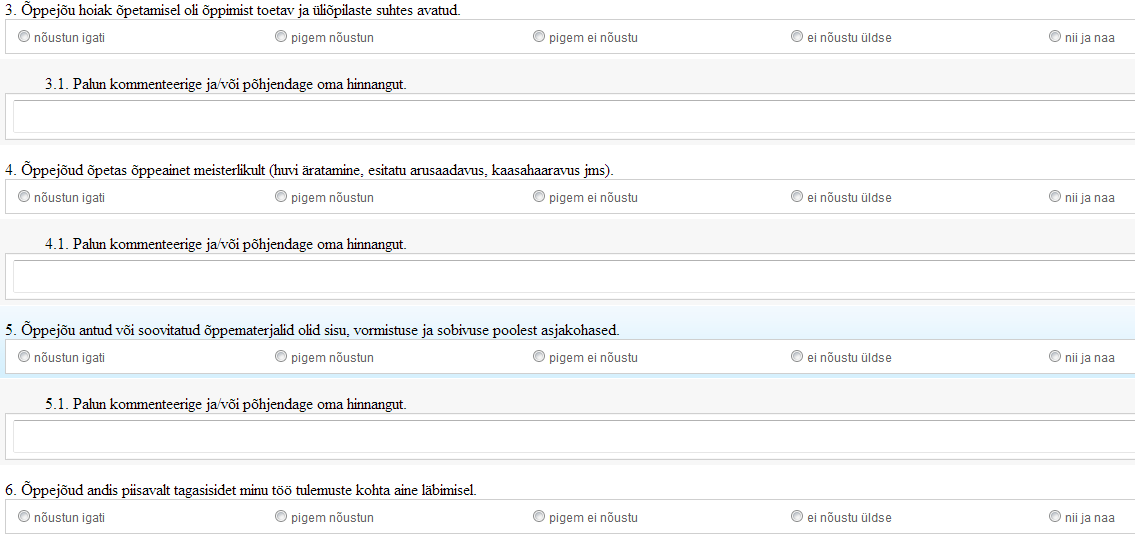
\includegraphics[width=0.8\textwidth]{ois_tagasiside_toodeldud.png}
\caption{Näide Tartu \"Ulikooli õppeinfo s\"usteemi tagasiside ankeedist, kus rakendatakse Likerti skaalat \cite{UT}}
\label{likert1}
\end{figure}

\begin{figure}[H]
\centering
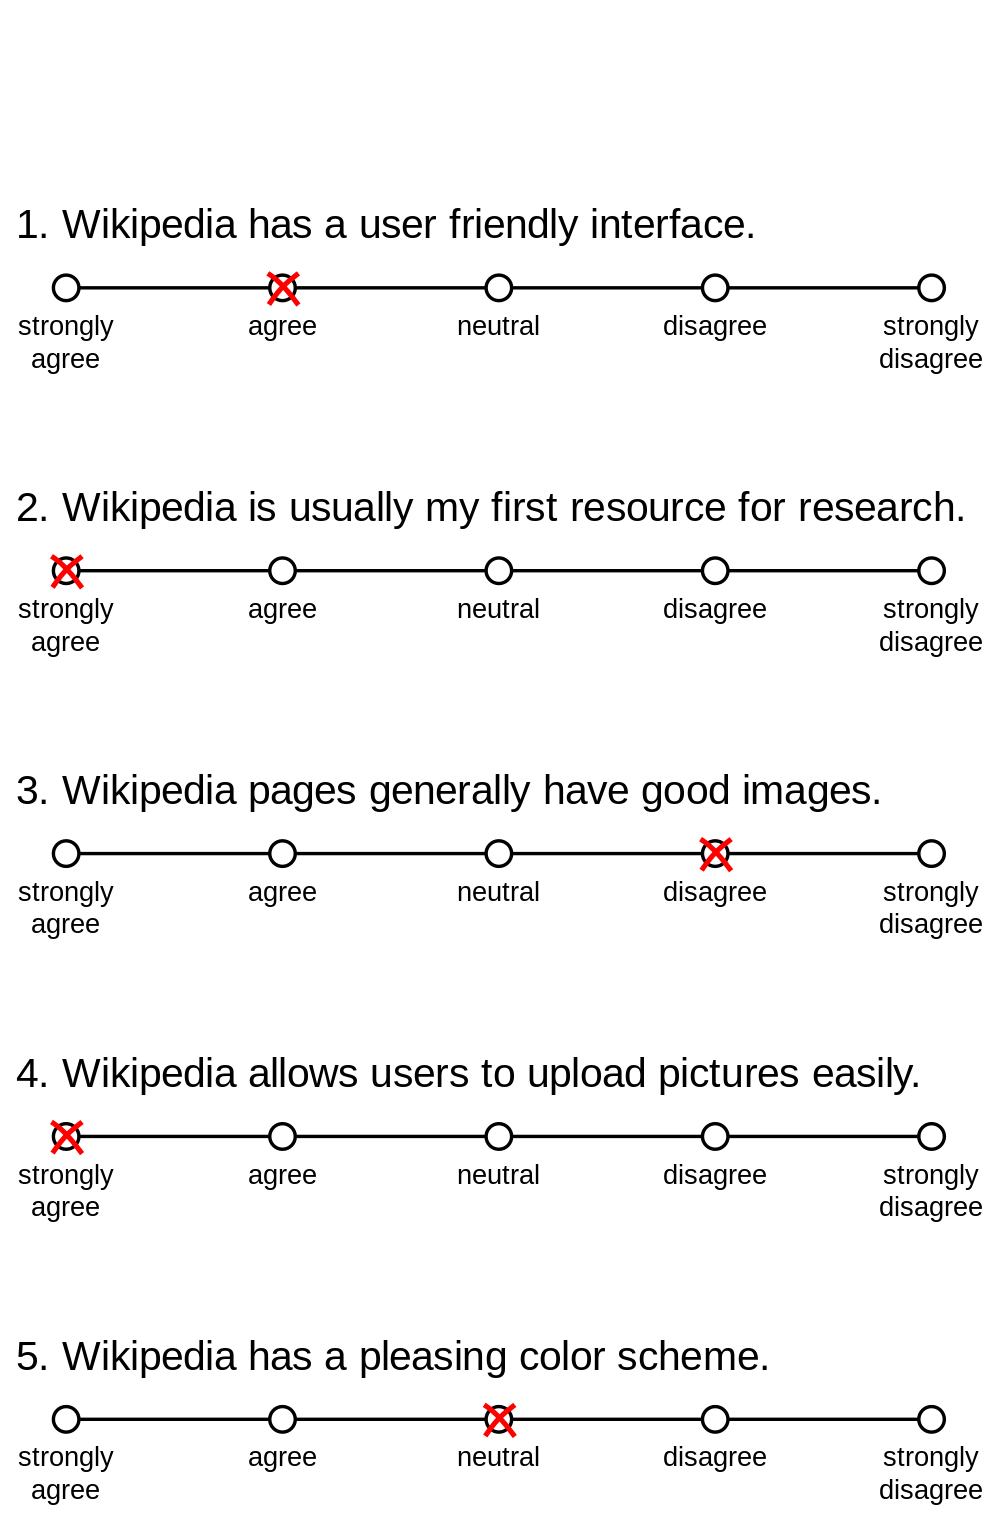
\includegraphics[width=0.5\textwidth, height = 0.7\textwidth]{Example_Likert_Scale.png}
\caption{Näide k\"usimustikust, kus on rakendatud Likerti skaalat; k\"usimused on paigutatud nende järjestikulisuse rõhutamiseks teljele\cite{Smith}}
\label{likert2}
\end{figure}



\pagebreak
\bibliography{mata_baka}{}
\bibliographystyle{plain}


\end{document}